% pythontex
\documentclass[xcolor=table,aspectratio=169,dvipsnames,english]{beamer}
\usepackage{bm}
\usepackage[utf8]{inputenc}
\usepackage{color}

\usepackage[british]{babel} % decent hyphenation, avoiding e.g. anal-ysis
\usepackage[iso]{isodate}
\usepackage{sansmath}
\usepackage{booktabs}
\usepackage{graphicx}
\usepackage{graphviz}
\usepackage{makecell}
\usepackage{minted}
\usepackage{siunitx}
\usepackage{subcaption}
\usepackage[section]{placeins}
\usepackage{amsfonts} % needed for \mathbb{} (Only works on capital letters!)
\usepackage{tikz}
\usetikzlibrary{shapes,snakes}
%\usetikzlibrary{shapes.geometric}

\usepackage{hyperref}
\usepackage{amsmath}
% Needs to be loaded after hyperref and amsmath
\usepackage{cleveref}

% new commands
\newcommand{\xdensity}{\textit{p}_x (\textbf{x})}
\newcommand{\udensity}{\textit{p}_u (\textbf{u})}
\newcommand{\transformer}{\tau(z_i;\textbf{h}_i)}
\newcommand{\conditioner}{c_i(\textbf{z}_{<1})}
\newcommand{\where}{\quad \text{where} \quad}
\newcommand{\xset}{\mathbb{X}}
\newcommand{\xseti}{\mathbb{X}^{(i)}}
\newcommand{\approxdistri}{q_{\phi_i}(\textbf{z}|\xseti)}
\newcommand{\approxdistr}{q_{\phi, \psi}(\textbf{z}|\xset)}
\newcommand{\truedistri}{p_{\theta}(\textbf{z}|\xseti)}
\newcommand{\truedistr}{p_{\theta}(\textbf{z}|\textbf{X})}
\newcommand{\elbo}{\mathcal{L}(\theta, \phi; \xseti)}
\newcommand{\xsubset}{\mathbb{X}_k}
\newcommand{\lmopoe}{\mathcal{L}_{MoPoE}(\theta, \phi; \xset)}
\newcommand{\powerset}{\mathcal{P}(\xset)}
\newcommand{\pFmean}{\mathcal{M}_{f_{\psi}}}
\newcommand{\DklTrueApprox}{D_{KL} \left( \approxdistr || \truedistr \right)}
\newcommand{\Mnfi}{\mathcal{M}_{f_{\psi}}\left( q_{\phi _i}(\textbf{z}|\textbf{x}_i) \right)}




% PythonTeX
\usepackage[autoprint=false, gobble=auto, keeptemps=all, pyfuture=all]{pythontex} % create figures on-line directly from python!
\usepackage{pgf}
\begin{pythontexcustomcode}[begin]{py}
import os, sys
almost_this_path = os.path.abspath(os.path.dirname(__file__))
this_path_base, _ = os.path.split(almost_this_path)
this_path = os.path.join(this_path_base,"pythontex")

from pylab import gcf
import matplotlib
import matplotlib.pyplot as plt

pytex.add_dependencies(os.path.join(this_path,'matplotlibrc.conf'))

plt.style.use(os.path.join(this_path,'matplotlibrc.conf'))

# Set the prefix used for figure labels
fig_label_prefix = 'fig'
# Track figure numbers to create unique auto-generated names
fig_count = 0

def figure_by_path(figure_path,textheight_frac=1,caption=None,label=None):
    latex_code = "\\begin{figure}\n"
    latex_code += "\\centering\\includegraphics[width={textheight_frac}\\textheight]{{{figure_path}}}\n".format(textheight_frac=textheight_frac,figure_path=figure_path)
    latex_code += "\\vspace{-2.5em}\n"
    latex_code += "\\caption{{{caption}}}\n".format(caption=caption)
    latex_code += "\\label{{fig:{label}}}\n".format(label=label)
    latex_code += "\\end{figure}\n"
    return latex_code

def save_fig(name='', legend=False, fig=None, ext='.pgf', fig_width=1, fig_height=1):
    '''
    Save the current figure (or `fig`) to file using `plt.save_fig()`.
    If called with no arguments, automatically generate a unique filename.
    Return the filename.
    '''
    # Get name (without extension) and extension
    if not name:
        global fig_count
        # Need underscores or other delimiters between `input_*` variables
        # to ensure uniqueness
        name = 'auto_fig_{}-{}'.format(pytex.id, fig_count)
        fig_count += 1
    else:
        if len(name) > 4 and name[:-4] in ['.pgf', '.svg', '.png', '.jpg']:
            name, ext = name.rsplit('.', 1)

    # Get current figure if figure isn't specified
    if not fig:
        fig = gcf()
    fig.set_size_inches(fig_width,fig_height)
    fig.savefig(name + ext)
    fig.clf()
    return name

def latex_environment(name, content='', option=''):
    '''
    Simple helper function to write the `\begin...\end` LaTeX block.
    '''
    return '\\vspace{-0.25cm}\\begin{%s}%s\n%s\n\\end{%s}' % (name, option, content, name)

def latex_figure(name=None, caption='', label='', width=1):
    ''''
    Auto wrap `name` in a LaTeX figure environment.
    Width is a fraction of `\textwidth`.
    '''
    if not name:
        name = save_fig()
    content = '\\centering\n'
    content += '\\makeatletter\\let\\input@path\\Ginput@path\\makeatother\n'
    content += '\\input{%s.pgf}\n' % name
    if not label:
        label = name
    if caption and not caption.rstrip().endswith('.'):
        caption += '.'
    if caption:
        # `\label` needs to be in `\caption` to avoid issues in some cases
        content += "\\caption{%s\\label{%s:%s}}\n" % (caption, fig_label_prefix, label)
    return latex_environment('figure', content, '[htp]')

pytex.bio_fignum = 0
#global pytex # try without this line
def bio_fig(gdd, fname=None, caption=None, label=None):
#        global pytex # and this one, should work
        if fname is None:
            fname = 'pythontex-files-pres/biopython_fig_{0}-{1}.pdf'.format(pytex.id, pytex.bio_fignum)
        gdd.write(fname, "PDF")
        template = '''
    \\begin{{figure}}
    \\centering
    \\includegraphics{{{fname}}}
    \\caption{{ {label} {caption} }}
    \\end{{figure}}
    '''
        if caption is None:
            caption = ''
        if label is None:
            label = ''
        else:
            if not label.startswith('fig:'):
                label = 'fig:' + label
            label = '\\label{{{0}}}'.format(label)
        template = template.format(fname=fname.rsplit('.', 1)[0], label=label, caption=caption)
        print(template)
        pytex.add_created(fname)
        pytex.bio_fignum += 1
        return template
\end{pythontexcustomcode}
\begin{pythontexcustomcode}[end]{py}
\end{pythontexcustomcode}

\begin{pythontexcustomcode}[begin]{py}
pytex.add_dependencies(
	'lib/utils.py',
	'lib/categorical.py',
	)
\end{pythontexcustomcode}
% Single-session PythonTeX codeblocks
\newcounter{pysessioncounter}
\newcommand{\sessionpy}{%
          \edef\sessionpysession{session\arabic{pysessioncounter}}%
            \stepcounter{pysessioncounter}%
              \expandafter\py\expandafter[\sessionpysession]}

% SIunitx customizations detect-all will use the current font for typesetting
\sisetup{per-mode=symbol, detect-all, range-units = single}
\newcommand\SIci[5]{\SI{#1}{#2}, {#3}CI: \SIrange{#4}{#5}{#2}}

% Fix for matplotlib PGF wonkiness which isn't interpreted correctly by pdflatex
\DeclareUnicodeCharacter{2212}{-}

%BIBLIOGRAPHY
% see https://mirror.foobar.to/CTAN/macros/latex/contrib/biblatex/doc/biblatex.pdf for available styles
\usepackage[backend=bibtex,style=authoryear,natbib=true]{biblatex}
\addbibresource{bib.bib}

% Article-specific configuration
\begin{pythontexcustomcode}[begin]{py}
DOC_STYLE="midterm_presentation/main.conf"
pytex.add_dependencies(
	DOC_STYLE,
	)
\end{pythontexcustomcode}

% Custom beamer styling and colors
\setbeamersize{text margin left=0.8em,text margin right=0.8em}
\setbeamertemplate{bibliography item}{\insertbiblabel}

\usecolortheme[RGB={199,199,199}]{structure}
\usetheme{default}

\captionsetup[figure]{labelformat=empty}

\definecolor{dy}{RGB}{202,202,0}
\definecolor{rsblue}{HTML}{00a3cc}
\definecolor{mg}{gray}{0.30}
\definecolor{lg}{gray}{0.60}
\definecolor{vlg}{gray}{0.78}
\definecolor{tlg}{gray}{0.88}

\setbeamercolor{caption name}{fg=lg}
\setbeamercolor{caption}{fg=lg}
\setbeamercolor{author}{fg=lg}
\setbeamercolor{institute}{fg=lg}
\setbeamercolor{date}{fg=lg}
\setbeamercolor{title}{fg=mg}
\setbeamertemplate{caption}{\centering\insertcaption\par}
\setbeamertemplate{navigation symbols}{}




\title[Multi Modal Generative Learning with Normalizing Flows]{Multi Modal Generative Learning with Normalizing Flows}
\subtitle{Midterm Presentation}
\author[Hendrik Klug]{Hendrik Klug}

\AtBeginEnvironment{frame}{\setcounter{footnote}{0}}

\begin{document}

    \begin{frame}
        \titlepage
    \end{frame}

    \begin{frame}{Global Theme}
        \centering
        \textbf{Finding a model that can learn a joint distribution of multiple data types.}

        \begin{figure}
            \resizebox{0.9\textwidth}{!}{%
                \py{pytex_printonly(script='midterm_presentation/scripts/generalidea_graph.py', data = '')}
            }
        \end{figure}
    \end{frame}

    \begin{frame}{Motivation}
        \begin{itemize}
            \item Can leverage the multiple data types present in the medical domain
            \item The training is self supervised $\rightarrow$ no labels required
            \item The latent representation can be used for classification
        \end{itemize}
    \end{frame}

    \begin{frame}{Background}
        The multimodal aspect has many advantages, but \textbf{combining the learned distributions for each modality into a joint latent distribution is still an open problem}.
        \begin{figure}
            \centering
            \resizebox{0.7\textwidth}{!}{%
                \begin{tikzpicture}[Mod1/.style={rectangle, draw=blue!60, fill=blue!5, very thick, minimum size=5mm},Mod2/.style={rectangle, draw=green!60, fill=green!5, very thick, minimum size=5mm},enc_mods/.style={circle, draw=gray!60, fill=gray!5, very thick, minimum size=10mm},magic/.style={rectangle, draw=red!60, fill=red!5, very thick, minimum size=20mm},]
                    \node[Mod1] (mod1) {$Mod_1$};
                    \node[below of=mod1] (points) {\ldots};
                    \node[enc_mods, right of=mod1, xshift=1.5cm] (q1) {$q_1$};
                    \node[Mod2, below of=points] (modn) {$Mod_n$};
                    \node[enc_mods, right of=modn, xshift=1.5cm] (q2) {$q_n$};
                    \node[below of=q1] (points) {\ldots};
                    \node[magic, right of=q1, yshift=-1cm, xshift=1.5cm] (magic) {\textbf{Magic!}};
                    \node[enc_mods, right of=magic, xshift=1.7cm] (joint) {Joint Distr};
                    \node[Mod1, right of=joint, xshift=1.7cm,yshift=+1cm] (rec_mod1) {$Mod_1$};
                    \node[right of=joint,xshift=1.7cm] (points) {\ldots};
                    \node[Mod2, right of=joint, xshift=1.7cm,yshift=-1cm] (rec_mod2) {$Mod_n$};
                    \draw[->] (mod1) -- node[anchor=south] {$enc_1$} (q1);
                    \draw[->] (q1) -- (magic);
                    \draw[->] (modn) -- node[anchor=south] {$enc_n$} (q2);
                    \draw[->] (q2) -- (magic);
                    \draw[->] (magic) -- (joint);
                    \draw[->] (joint) edge[bend left=20] node[anchor=south] {$dec_1$} (rec_mod1);
                    \draw[->] (joint) edge[bend right=20] node[anchor=north] {$dec_n$} (rec_mod2);
                \end{tikzpicture}
            }
        \end{figure}
    \end{frame}

    \begin{frame}{The Mixture-of-Products-of-Experts-VAE (MoPoE)}
        The MoPoE is a method from \cite{thomas_gener-ELBO}, which is a combination of:
        \begin{itemize}
            \item The Product-of-Experts (PoE) from \cite{wu2018multimodal}
            \item The Mixture-of-Experts (MoE) from \cite{shi2019variational}
        \end{itemize}
    \end{frame}

    \begin{frame}{The Mixture-of-Products-of-Experts-VAE (MoPoE)}
        \begin{figure}
            \centering
            \resizebox{0.9\textwidth}{!}{%
                \py{pytex_printonly(script='midterm_presentation/scripts/mopoe_graph.py', data = '')}
            }
        \end{figure}

        \begin{small}
            \begin{equation*}
                \log p_{\theta}(\mathbb{X}) \geq \eqlmopoe
            \end{equation*}

            \begin{equation*}
                \text{with:}\ \tilde{q}_{\phi}(\textbf{z}|\xsubset)=PoE(\{q_{\phi_j}(\textbf{z}|\textbf{x}_j) \forall \textbf{x}_j \in \xsubset\}) \propto \prod _{\textbf{x}_j \in \xsubset}q_{\phi_j}(\textbf{z}|\textbf{x}_j)
            \end{equation*}

        \end{small}

    \end{frame}

    \begin{frame}{Generalizing with the generalized $f$-mean}
        Both the PoE and the MoE can be generalized since both are special cases of the generalized f-mean \footcite{niculescu_convex_2018}:
        $$\mathcal{M}_{f}\left( \textbf{p} \right) = f^{-1}\left( \frac{1}{N} \sum ^N _{i=1} f(\textbf{p}_i)) \right)$$

        \textbf{Basic idea:}
        Make the fusion of the uni modal latent spaces more flexible by using an f-mean.
    \end{frame}

    \begin{frame}{Generalizing with the generalized $f$-mean}
        \begin{figure}
            \centering
            \resizebox{0.7\textwidth}{!}{%
                \begin{tikzpicture}[Mod1/.style={rectangle, draw=blue!60, fill=blue!5, very thick, minimum size=5mm},Mod2/.style={rectangle, draw=green!60, fill=green!5, very thick, minimum size=5mm},enc_mods/.style={circle, draw=gray!60, fill=gray!5, very thick, minimum size=10mm},magic/.style={rectangle, draw=red!60, fill=red!5, very thick, minimum size=20mm},]
                    \node[Mod1] (mod1) {$Mod_1$};
                    \node[below of=mod1] (points) {\ldots};
                    \node[enc_mods, right of=mod1, xshift=1.5cm] (q1) {$q_1$};
                    \node[Mod2, below of=points] (modn) {$Mod_n$};
                    \node[enc_mods, right of=modn, xshift=1.5cm] (q2) {$q_n$};
                    \node[below of=q1] (points) {\ldots};
                    \node[magic, right of=q1, yshift=-1cm, xshift=1.5cm] (magic) {\textbf{Magic!}};
                    \node[enc_mods, right of=magic, xshift=1.7cm] (joint) {Joint Distr};
                    \node[Mod1, right of=joint, xshift=1.7cm,yshift=+1cm] (rec_mod1) {$Mod_1$};
                    \node[right of=joint,xshift=1.7cm] (points) {\ldots};
                    \node[Mod2, right of=joint, xshift=1.7cm,yshift=-1cm] (rec_mod2) {$Mod_n$};
                    \draw[->] (mod1) -- node[anchor=south] {$enc_1$} (q1);
                    \draw[->] (q1) -- (magic);
                    \draw[->] (modn) -- node[anchor=south] {$enc_n$} (q2);
                    \draw[->] (q2) -- (magic);
                    \draw[->] (magic) -- (joint);
                    \draw[->] (joint) edge[bend left=20] node[anchor=south] {$dec_1$} (rec_mod1);
                    \draw[->] (joint) edge[bend right=20] node[anchor=north] {$dec_n$} (rec_mod2);
                \end{tikzpicture}
            }
        \end{figure}
    \end{frame}

    \begin{frame}{Generalizing with the generalized $f$-mean}
        \begin{figure}
            \centering
            \resizebox{0.7\textwidth}{!}{%
                \begin{tikzpicture}[Mod1/.style={rectangle, draw=blue!60, fill=blue!5, very thick, minimum size=5mm},Mod2/.style={rectangle, draw=green!60, fill=green!5, very thick, minimum size=5mm},enc_mods/.style={circle, draw=gray!60, fill=gray!5, very thick, minimum size=10mm},magic/.style={rectangle, draw=red!60, fill=red!5, very thick, minimum size=20mm},]
                    \node[Mod1] (mod1) {$Mod_1$};
                    \node[below of=mod1] (points) {\ldots};
                    \node[enc_mods, right of=mod1, xshift=1.5cm] (q1) {$q_1$};
                    \node[Mod2, below of=points] (modn) {$Mod_n$};
                    \node[enc_mods, right of=modn, xshift=1.5cm] (q2) {$q_n$};
                    \node[below of=q1] (points) {\ldots};
                    \node[magic, right of=q1, yshift=-1cm, xshift=1.5cm] (magic) {\textbf{$f$-Mean}};
                    \node[enc_mods, right of=magic, xshift=1.7cm] (joint) {Joint Distr};
                    \node[Mod1, right of=joint, xshift=1.7cm,yshift=+1cm] (rec_mod1) {$Mod_1$};
                    \node[right of=joint,xshift=1.7cm] (points) {\ldots};
                    \node[Mod2, right of=joint, xshift=1.7cm,yshift=-1cm] (rec_mod2) {$Mod_n$};
                    \draw[->] (mod1) -- node[anchor=south] {$enc_1$} (q1);
                    \draw[->] (q1) -- (magic);
                    \draw[->] (modn) -- node[anchor=south] {$enc_n$} (q2);
                    \draw[->] (q2) -- (magic);
                    \draw[->] (magic) -- (joint);
                    \draw[->] (joint) edge[bend left=20] node[anchor=south] {$dec_1$} (rec_mod1);
                    \draw[->] (joint) edge[bend right=20] node[anchor=north] {$dec_n$} (rec_mod2);
                \end{tikzpicture}
            }
        \end{figure}
    \end{frame}

    \begin{frame}{Generalizing with the generalized $f$-mean}
        $f$ can be anything as long as it is injective
        $\rightarrow$ $f$ can be parameterized as a normalizing flow\footcite{papamakarios_normalizing_2019} $f_{\psi}$
        $$\mathcal{M}_{f_{\psi}}\left( \textbf{p} \right) = f_{\psi}^{-1}\left( \frac{1}{N} \sum ^N _{i=1} f_{\psi}(\textbf{p}_i)) \right)$$
    \end{frame}

    \begin{frame}{Normalizing flows}
    Normalizing flows represent an approach for defining invertible and differentiable transformations of probability distributions.
    They are widely used for:
    \begin{itemize}
        \item generative modeling \citep[\textbf{GLOW}, \textbf{Real NVP}]{kingma_glow_2018, dinh_density_2017}
        \item variational inference (\cite{rezende_variational_2016, berg_sylvester_2019})
    \end{itemize}
\end{frame}

\begin{frame}{Implementation of the Normalizing Flows}
    As implementation of the normalizing flows, I use the coupling block \citep[Real NVP]{dinh_density_2017} from the Framework for Easily Invertible Architectures (FrEIA) \footnote{https://github.com/VLL-HD/FrEIA}.
    \begin{figure}
        \centering
        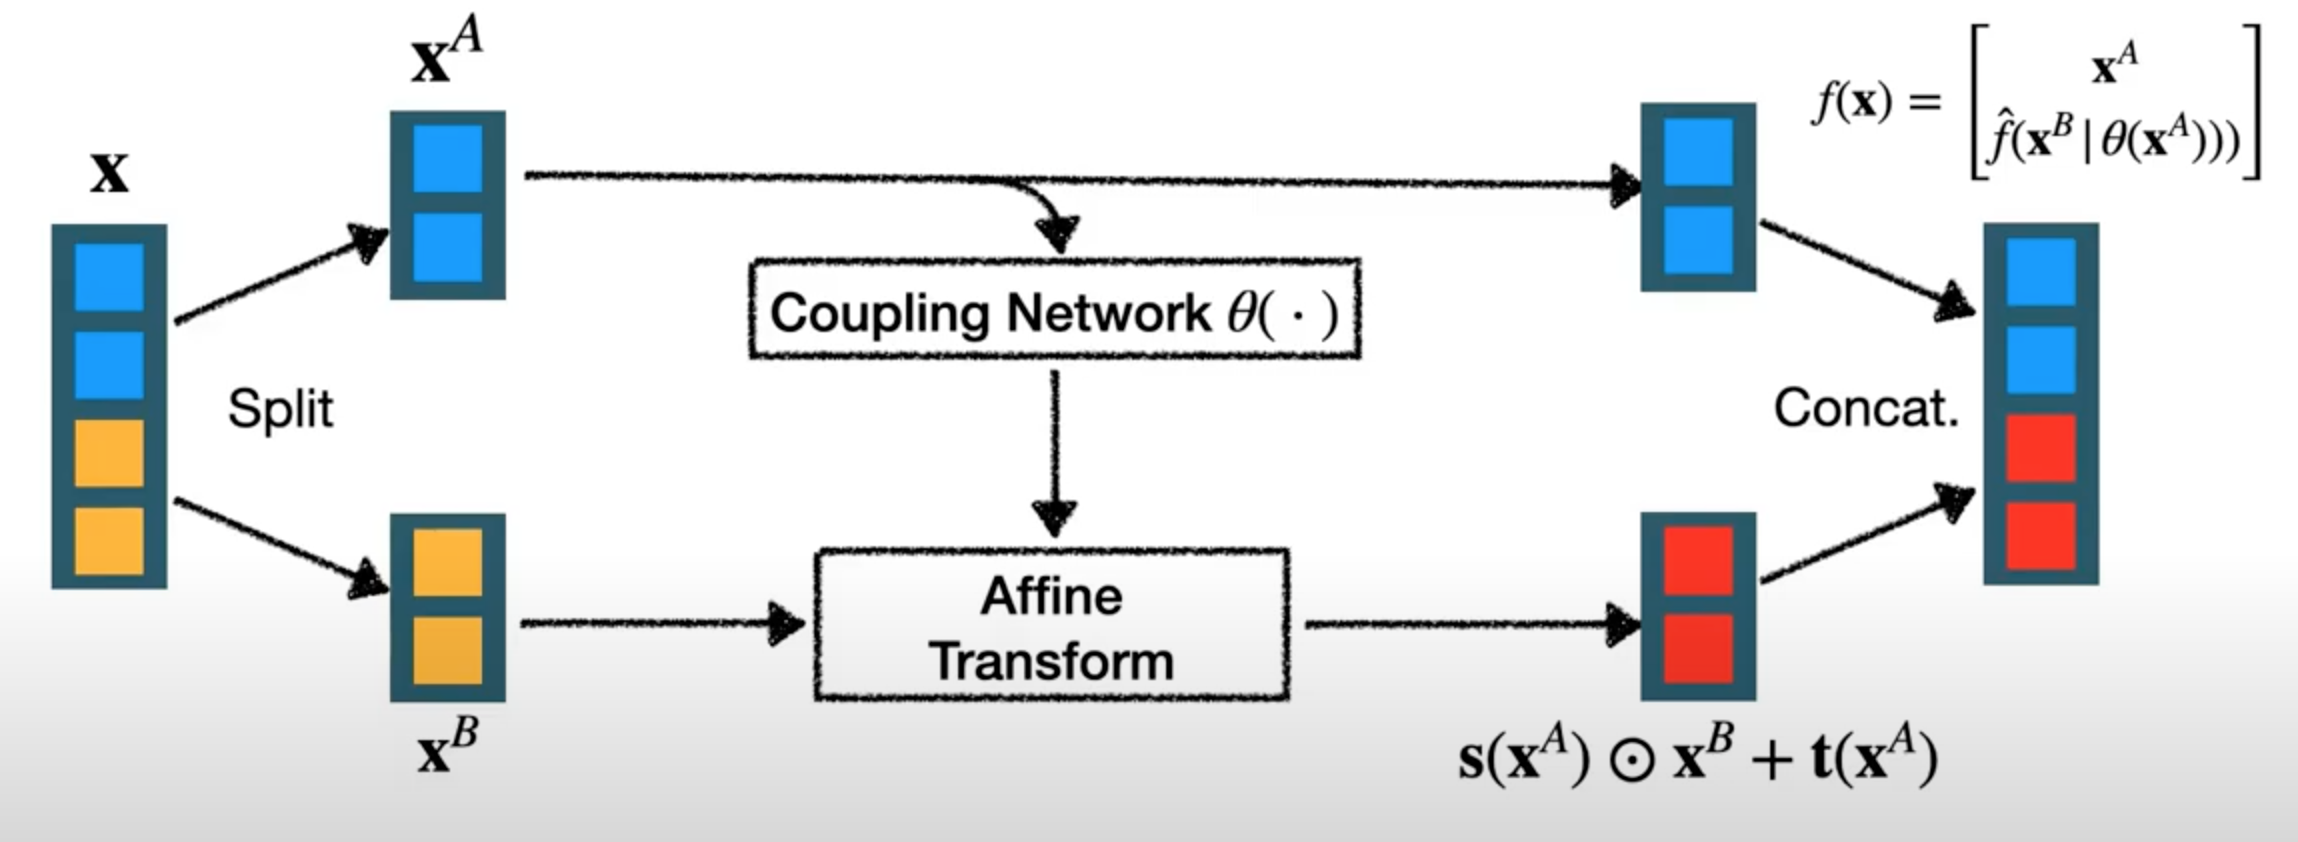
\includegraphics[width = 0.8\textwidth]{midterm_presentation/coupling_flow}
        \caption{\tiny{Taken from https://youtu.be/u3vVyFVU\_lI}}
    \end{figure}
\end{frame}

\begin{frame}{The polymnist dataset}
    \begin{figure}
        \centering
        \includegraphics[width=0.8\textwidth]{data/polymnist_example}
    \end{figure}
    Properties:
    \begin{itemize}
        \item Very simple class representation (almost the same across all modalities and very simple)
        \item More difficult modality specific representation (background of \textit{Mod 0} and \textit{Mod 2} is more complex)
    \end{itemize}
\end{frame}

\begin{frame}{Difficulties}
    The main difficulty comes from the fact that the $f$-mean of Normal distributions is not a Normal distribution.\\
    $\rightarrow$ The KL-divergence is hard to compute.\\
    \begin{equation*}
        \log p_{\theta}(\mathbb{X}) \geq \mathcal{L}(\theta, \phi; \xset):= \mathbb{E}_{q_{\phi}(\textbf{z}|\mathbb{X})}[\log (p_{\theta}(\mathbb{X}|\textbf{z}))] - D_{KL}\biggl(  q_{\phi}(\textbf{z}|\mathbb{X})\ ||\ p_{\theta}(\textbf{z})\biggr)
    \end{equation*}
\end{frame}

\begin{frame}{KL-divergence of $f$-mean}
    \textbf{3 options}:

    \begin{enumerate}[<+->]
        \item Instead of mixing distributions $\mathcal{M}_{f_{\psi}}(\mathcal{N}(\mu _i, \sigma_i^2))$, mix the parameters:\\
        $\mu_{joint} = \mathcal{M}_{f_{\psi}}(\mu _i)$, $\sigma_{joint}^2 = \mathcal{M}_{f_{\psi}}( \sigma_i^2)$ $\rightarrow q_{\phi_{joint}} \sim \mathcal{N}\left(  f_{\mu}^{-1}(\sum ^M \frac{f_{\mu}(\mu_i)}{M}),f_{\sigma}^{-1}(\sum ^M \frac{f_{\sigma}(\sigma_i^2)}{M})\right)$
        \item Instead of computing the KL-divergence in closed form, calculate it by sampling from the posterior, i.e. compare k samples from the posterior with k samples from the prior
        \item \only<.>{Find an upper bound $ D^{\prime}_{KL} \geq D_{KL}(\mathcal{M}_{f_{\psi}}(\mathcal{N}(\mu _i, \sigma_i^2))\ ||\  p_{\theta})$}\only<+->{\sout{Find an upper bound $ D^{\prime}_{KL} \geq D_{KL}(\mathcal{M}_{f_{\psi}}(\mathcal{N}(\mu _i, \sigma_i^2))\ ||\  p_{\theta})$}}

    \end{enumerate}
\end{frame}

\begin{frame}{Parameter $f$-Mean VAE}
    \begin{figure}
        \centering
        \resizebox{0.9\textwidth}{!}{%
            \py{pytex_printonly(script='midterm_presentation/scripts/pgfm_graph.py', data = '')}
        }
    \end{figure}

    \begin{small}
        \begin{equation*}
            \log p_{\theta}(\mathbb{X}) \geq \eqlpgfm
        \end{equation*}

        \begin{equation*}
            \text{with:}\ \tilde{q}_{\phi_{12}} \sim \mathcal{N}\left(  f_{\mu}^{-1}(\frac{f_{\mu}(\mu_1) + f_{\mu}(\mu_2)}{2}),f_{\sigma}^{-1}(\frac{f_{\sigma}(\sigma_1^2) + f_{\sigma}(\sigma_2^2)}{2})\right)
        \end{equation*}

    \end{small}

\end{frame}

\begin{frame}{Parameter $f$-Mean VAE}
    \begin{figure}
        \centering
        \resizebox{0.9\textwidth}{!}{%
            \py{pytex_printonly(script='midterm_presentation/scripts/pgfm_graph_.py', data = '')}
        }
    \end{figure}
\end{frame}

\begin{frame}{Mixture of Parameter $f$-Mean VAE}
    \begin{figure}
        \centering
        \resizebox{0.9\textwidth}{!}{%
            \py{pytex_printonly(script='midterm_presentation/scripts/mopgfm_graph.py', data = '')}
        }
    \end{figure}

    \begin{small}
        \begin{equation*}
            \log p_{\theta}(\mathbb{X}) \geq \eqlmopgfm
        \end{equation*}

        \begin{equation*}
            \text{with:}\ \tilde{q}_{\phi_{i}} \sim \mathcal{N}\left(  f_{\mu}^{-1}(\sum ^S _{i = 0}\frac{f_{\mu}(\mu_i)}{S}),f_{\sigma}^{-1}(\sum ^S _{i = 0}\frac{f_{\sigma}(\sigma_i^2)}{S})\right)
        \end{equation*}
    \end{small}
\end{frame}

\begin{frame}{Importance Weighted $f$-Mean VAE}
    Instead of computing the KL-divergence in closed form, calculate it by sampling from the posterior following the procedure from the importance weighted autoencoder \citep{burda_importance_2016, shi_variational_2019}.
    \begin{equation*}
        \log p(x) \geq \mathbb{E}_{z_1,\ldots,z_K \sim q_{\phi}(z|x)}\left[ \log \frac{1}{K} \sum ^K _{i=1} \frac{p_{\theta}(x|z_i)p_{\theta}(z)}{q_{\phi}(z_i| x)} \right]\\
        := \mathcal{L}_K
    \end{equation*}
\end{frame}

\begin{frame}{Known results \citep{nowozin_debiasing_2018}}
    \begin{enumerate}
        \item ELBO recovery:
        \begin{equation*}
            ELBO = \mathcal{L}_1
        \end{equation*}
        \item Consistency: $\lim _{K \rightarrow \inf} \mathcal{L}_K = \log p(x)$
        \item Stochastic monotonicity:
        \begin{equation*}
            \mathcal{L}_E = \mathcal{L}_1 \leq \mathcal{L}_2 \leq \ldots \leq \log p(x)
        \end{equation*}
    \end{enumerate}
\end{frame}

\begin{frame}{Mixture of $f$-Mean}
    \begin{figure}
        \centering
        \resizebox{0.9\textwidth}{!}{%
            \py{pytex_printonly(script='midterm_presentation/scripts/mogfm_graph.py', data = '')}
        }
    \end{figure}

    \begin{equation*}
        \mathcal{L}_{mogfm} := \mathbb{E}_{q_{\phi}(z^{\prime}|\mathbb{X})}\left[ \log p_{\theta}(\mathbb{X}|z^{\prime}) \right] - D_{KL}(q_{\phi}(z|\mathbb{X})\ ||\ P_{\theta}(z))
    \end{equation*}

    Where the KL-divergence is calculated with $K$ samples from $q_{\phi}(z|\mathbb{X})$ and from the prior $q_{\theta}$:
    \begin{equation*}
        D_{KL} = \text{mean}(\left\{ l_1,\ldots,l_N \right\}) \text{, with } l_n=y_n\cdot(\log y_n -x_n) \text{ and } x_n \sim q_{\phi}(z|\mathbb{X}); y_n \sim q_{\theta}
    \end{equation*}
\end{frame}



    \begin{frame}{Preliminary Results}{Log-likelihoods}
    \py{
        pytex_tab(
        script='midterm_presentation/scripts/lhood_tab.py',
        options_pre='\\centering \\resizebox{0.9\\textwidth}{!}{',
        options_post='}',
        caption='Test set log-likelihoods.',
        )
    }
\end{frame}

\begin{frame}{Preliminary Results}{Latent Representation Evaluation}
    \py{
        pytex_tab(
        script='midterm_presentation/scripts/lr_eval_tab.py',
        options_pre='\\centering \\resizebox{0.9\\textwidth}{!}{',
        options_post='}',
        caption='Linear classification accuracy of latent representations for the Test set.\\
        ',
        )
    }
\end{frame}

\begin{frame}{Preliminary Results}{Generation Coherence Evaluation}
    \py{
        pytex_tab(
        script='midterm_presentation/scripts/gen_eval_tab.py',
        options_pre='\\centering \\resizebox{0.9\\textwidth}{!}{',
        options_post='}',
        caption='Generation coherence for the Test set.
        ',
        )
    }
\end{frame}


\begin{frame}{Preliminary Results}{Generation Quality Evaluation}
    \py{
        pytex_tab(
        script='midterm_presentation/scripts/prd_tab.py',
        options_pre='\\centering \\resizebox{0.9\\textwidth}{!}{',
        options_post='}',
        caption='Area under the Precision and Recall curve of the PRD score \citep{precision_recall_distributions}.
        ',
        )
    }
\end{frame}


%\begin{frame}{Preliminary Results}{Qualitative Evaluation}
%    \begin{figure}
%        \centering
%        \resizebox{0.9\textwidth}{!}{%
%            \py{boilerplate.make_cond_gen_fig(which='m1_m2__m1', methods=['mopoe','mopgfm', 'mogfm'])}
%        }
%    \end{figure}
%\end{frame}

\begin{frame}{Preliminary Results}{Qualitative Evaluation}
    \begin{figure}
        \centering
        \resizebox{0.9\textwidth}{!}{%
            \py{boilerplate.make_cond_gen_fig(which='m1_m2__m2', methods=['mopoe','mopgfm', 'mogfm'])}
        }
    \end{figure}
\end{frame}

\begin{frame}{Preliminary Results}{Qualitative Evaluation}
    \begin{figure}
        \centering
        \resizebox{0.9\textwidth}{!}{%
            \py{boilerplate.make_cond_gen_fig(which='m0_m1__m2', methods=['mopoe','mopgfm', 'mogfm'])}
        }
    \end{figure}
\end{frame}



%\begin{frame}{Preliminary Results}{Qualitative Evaluation}
%    \begin{figure}
%        \centering
%        \resizebox{0.9\textwidth}{!}{%
%            \py{boilerplate.make_cond_gen_fig(which='m0_m1__m0', methods=['mopoe','mopgfm', 'mogfm'])}
%        }
%    \end{figure}
%\end{frame}

    \begin{frame}{Mixture of Flow of Product of Experts VAE}
        Normalizing Flows can also be used to construct \textbf{flexible} and \textbf{arbitrarily complex} latent distributions, by passing the latent distribution through a series of $F$ invertible transformations \citep{rezende_variational_2016, berg_sylvester_2019}:
        \begin{equation*}
            z_F = f_F \circ \ldots \circ f_2 \circ f_1(z_0 \sim q_{\phi}(z|X))
        \end{equation*}
        \begin{equation*}
            \ln q_F(z_F) = \ln q_0 (z_0) - \sum _{f=1} ^{F}\ln \left|  \det \frac{df_f}{dz_{f-1}}\right|
        \end{equation*}
        such that:
        \begin{small}

            \begin{equation*}
                \mathcal{L}_{mofop} := \mathbb{E}_{q_{\phi}(\textbf{z}|\mathbb{X})}[\log (p_{\theta}(\mathbb{X}|\textbf{z}))] - D_{KL}\biggl( \frac{1}{2^M} \sum _{\mathbb{X}_k \in \mathcal{P}(\mathbb{X})} \tilde{q}_{\phi}(\textbf{z}|\mathbb{X}_k)\ ||\ p_{\theta}(\textbf{z})\biggr)
            \end{equation*}

            \begin{equation*}
                D_{KL}(\tilde{q}_{F; \phi_i}(\textbf{z}_{F,i}|X)\ ||\ P_{\theta}(z)) =
                \mathbb{E}_{\tilde{q}_{0; \phi_i}} \left[ \log \tilde{q}_{0; \phi_i}(\textbf{z}_0|X) -\log p_{\theta}(z) \right] - \mathbb{E}_{\tilde{q}_{0; \phi_i}}\left[ \sum_{f=1}^{F} \log \left| \det \left( \frac{d f_f (\textbf{z}_{f-1}; \lambda_f)}{d\textbf{z}_{f-1}} \right) \right| \right]
            \end{equation*}
        \end{small}

    \end{frame}

    \begin{frame}{Mixture of Flow of Product of Experts VAE}
        \begin{figure}
            \centering
            \resizebox{0.9\textwidth}{!}{%
                \py{pytex_printonly(script='midterm_presentation/scripts/mofop_graph.py', data = '')}
            }
        \end{figure}
        \begin{footnotesize}
            \begin{equation*}
                \mathcal{L}_{mofop} := \mathbb{E}_{q_{\phi}(\textbf{z}|\mathbb{X})}[\log (p_{\theta}(\mathbb{X}|\textbf{z}))] - \frac{1}{2^M} \left( \sum_{\mathbb{X}_k \in \mathcal{P}(\mathbb{X})} D_{KL}(q_{0; \phi}(\textbf{z}_0|X)\ ||\ p_{\theta}(\textbf{z})) - \mathbb{E}_{\tilde{q}_{0}}\left[ \sum_{f=1}^{F} \log \left| \det \left( \frac{d f_f (\textbf{z}_{f-1}; \lambda_f)}{d\textbf{z}_{f-1}} \right) \right| \right] \right)
            \end{equation*}
        \end{footnotesize}
    \end{frame}

    \begin{frame}{To Do}
        \begin{itemize}
            \item Continue the work in progress of the current methods
            \item Implement and test Importance Weighted MoPoE
            \item Find an upper bound of the KL-Divergence
            \item Evaluate methods on other datasets (MNIST-SVHN-Text, MIMIC-CXR)
            \vspace{3cm}
            \pause
%            \item Implement and test a method where the joint latent distribution is passed through a normalizing flow
            \item Write Thesis
        \end{itemize}
    \end{frame}



    % Disadvantages: slow
    %%%%%%%%%%%%%%%%%%%%%%%%%%%%%%%%%%%%%%%%%%%%%%%%%%%%%%%%%%%%%%%%%%%%%%%%%%%%%%%%%%%%%%%%%%%%%%%%%%%%%%%%%%%%%%%%%%%%

    \begin{frame}
        \centering
        \textbf{\huge{Thank you!}}
    \end{frame}


    \begin{frame}[allowframebreaks]
        \frametitle{References}
        \setbeamertemplate{bibliography item}{}
        \renewcommand*{\bibfont}{\tiny}
        \printbibliography
    \end{frame}

    
\begin{frame}{Parameters}
    \py{
        pytex_tab(
        script='midterm_presentation/scripts/params_tab.py',
        options_pre='\\centering \\resizebox{0.9\\textwidth}{!}{',
        options_post='}',
        caption='Hyperparameters that were selected using a hyperparameter search with Optuna \citep{akiba_optuna_2019}.',
        )
    }

\end{frame}



\begin{frame}{The mixture of $f$-mean}
\begin{equation*}
        \begin{split}
        & \mathbb{E}_{q_{\phi}(\textbf{z}|\mathbb{X})}[\log (p_{\theta}(\mathbb{X}|\textbf{z}))] - D_{KL}\biggl( \frac{1}{2^M} \sum _{\mathbb{X}_k \in \mathcal{P}(\mathbb{X})} \tilde{q}_{\phi}(\textbf{z}|\mathbb{X}_k)\ ||\ p_{\theta}(\textbf{z})\biggr)\\
        & \geq \mathbb{E}_{q_{\phi}(\textbf{z}|\mathbb{X})}[\log (p_{\theta}(\mathbb{X}|\textbf{z}))] - \frac{1}{2^M} \sum _{\mathbb{X}_k \in \mathcal{P}(\mathbb{X})}  D_{KL}\biggl(  \tilde{q}_{\phi}(\textbf{z}|\mathbb{X}_k)\ ||\ p_{\theta}(\textbf{z})\biggr) \\
        & \approx \mathbb{E}_{q_{\phi}(\textbf{z}|\mathbb{X})}[\log (p_{\theta}(\mathbb{X}|\textbf{z}))] -\frac{1}{2^M} \sum _{\mathbb{X}_k \in \mathcal{P}(\mathbb{X})}\text{mean}(\left\{ l_1,\ldots,l_N \right\}) \\
        & \text{with } l_n=y_n\cdot(\log y_n -x_n) \text{ and } x_n \sim q_{\phi}(z|\mathbb{X}_k);\ y_n \sim q_{\theta}\\
        & \text{and } \textbf{z} ^{\prime} = MoE(\{\frac{1}{K} \sum ^K _{i=1} (z_i \sim \tilde{q}_{\phi}(z|\mathbb{X}_k))\ \forall\ \mathbb{X}_k \in \mathcal{P}(\mathbb{X})\})
    \end{split}
\end{equation*}
\end{frame}



\begin{frame}{Preliminary Results}{Qualitative Evaluation}
    \begin{figure}
        \centering
        \resizebox{0.9\textwidth}{!}{%
            \py{boilerplate.make_cond_gen_fig(which='m1_m2__m0', methods=['mopoe','mopgfm', 'mogfm'])}
        }
    \end{figure}
\end{frame}

\begin{frame}{Preliminary Results}{Qualitative Evaluation}
    \begin{figure}
        \centering
        \resizebox{0.85\textwidth}{!}{%
            \py{boilerplate.make_cond_gen_fig(which='m0_m1_m2__m2', methods=['mopoe','mopgfm', 'mogfm'])}
        }
    \end{figure}
\end{frame}



\begin{frame}{Preliminary Results}{Qualitative Evaluation}
    \begin{figure}
        \centering
        \resizebox{0.9\textwidth}{!}{%
            \py{boilerplate.make_cond_gen_fig(which='m1_m2__m1', methods=['mopoe','mopgfm', 'mogfm'])}
        }
    \end{figure}
\end{frame}



\begin{frame}
    The KL-divergence of the sum of random variables is not convex.\\

    \textit{Proof:}\\
    Let $q_1, q_2, q_p \sim \mathcal{N}(0, \textbf{I})$.\\
    Then $D_{KL}(q_1||q_p) = D_{KL}(q_2||q_p) = 0$.\\
    But $D_{KL}(\frac{q_1 + q_2}{2}||q_p) = D_{KL}(q_{12}||q_p) > 0$ with $q_{12} \sim \mathcal{N}(\frac{1}{2}(\mu_1 + \mu_2), (\frac{\sigma_1}{4})^2+(\frac{\sigma_2}{4})^2))$
\end{frame}

\end{document}
